\documentclass[10pt]{article}
\usepackage[polish]{babel}
\usepackage[utf8]{inputenc}
\usepackage[T1]{fontenc}
\usepackage{amsmath}
\usepackage{amsfonts}
\usepackage{amssymb}
\usepackage[version=4]{mhchem}
\usepackage{stmaryrd}
\usepackage{graphicx}
\usepackage[export]{adjustbox}
\graphicspath{ {./images/} }

\title{LIGA MATEMATYCZNA \\
 im. Zdzisława Matuskiego \\
 LISTOPAD 2016 \\
 SZKOŁA PODSTAWOWA }

\author{}
\date{}


\begin{document}
\maketitle
\section*{ZADANIE 1.}
Adam i Bartek założyli się o jedną czekoladę. Jeżeli Adam wygra zakład, to będzie miał trzy razy tyle czekolad, co Bartek. Jeżeli Adam przegra, to będzie miał tylko dwa razy więcej czekolad niż Bartek. Ile czekolad miał każdy z nich na początku?

\section*{ZADANIE 2.}
W kwadracie o polu 64 wybrano punkt \(M\) i połączono go ze wszystkimi wierzchołkami. Powstały w ten sposób cztery trójkąty, z których jeden ma pole 12, a inny ma pole 24 . Podaj odległości punktu \(M\) od wszystkich boków kwadratu.

\section*{ZADANIE 3.}
Iloczyn dwóch liczb dwucyfrowych jest równy 525. Zaokrąglono te liczby do pełnych dziesiątek. Iloczyn tych zaokrągleń jest równy 600 . Znajdź początkowe liczby.

\section*{ZADANIE 4.}
Ile jest liczb dziesięciocyfrowych o sumie cyfr równej 3?

\section*{ZADANIE 5.}
Obwód największego z narysowanych kwadratów jest równy 80, a pole najmniejszego - 16. Oblicz obwód całej figury oraz pola kwadratów \(B\) i \(C\).\\
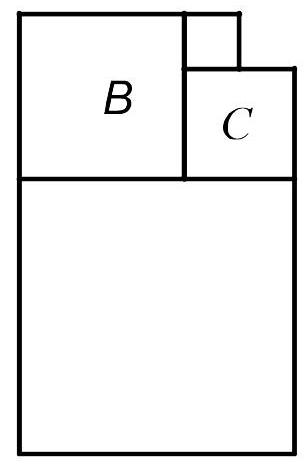
\includegraphics[max width=\textwidth, center]{2024_11_21_060a5cad90845cd37d9ag-1}


\end{document}